%************************************************
\chapter{Hypotheses and Counterfactual Knowledge}
\label{chapter:hypotheses_and_counterfactual_knowledge}
%************************************************

\section{Hypotheses}

I have previously described grounded factual knowledge that has an
unquestionable basis in symbolic perceptions.  Now, I will describe
how hypothetical causal models are abstracted from this factual
knowledge in order to create counterfactual knowledge, which keeps
this factual references so that it can be debugged when it is wrong.

\section{Hypothesis Space}

\cite{mitchell:1997} presents a general formalism for learning
hypotheses from sets of ground truth examples.  He describes a
function approximation approach to the discrimination problem of
predicting a binary value given a set of binary features.  In order to
keep the model of learning as general as possible, Mitchell introduces
the concept of a \emph{hypothesis space}.  Given a language for
describing hypotheses, the hypothesis space includes all possible
expressions in this language.  The hypothesis language can be
arbitrarily general, but in order to demonstrate my thesis about
reflective thinking, I make the simplifying assumption that this
language is simply based on the logical ``and'' expression.  This is
called the \emph{conjunctive hypothesis space}.  The conjunctive
hypothesis space consists of all logical conjunctions of the input
features.

\section{The General-to-Specific Ordering of Hypotheses}

\begin{definition}
\emph{Let $h_j$ and $h_k$ be Boolean-valued functions defined over
  $X$. Then $h_j$ is more-general-than-or-equal-to $h_k$ (written
  $h_j\ \geq_g\ h_k$) if and only if
\begin{equation*}
\forall_{x \in X}, [(h_k(x) = 1) \rightarrow (h_j(x) = 1)]
\end{equation*}
}\end{definition}

Depending on the choice of hypothesis language, it is not always
trivial to determine whether one hypothesis is more general than
another.  All non-redundant hypotheses in the conjunctive hypothesis
space of four input variables is shown as ordered in a generalization
lattice in
{\mbox{\autoref{figure:example_conjunctive_hypothesis_space}}}.
\begin{figure}
\center
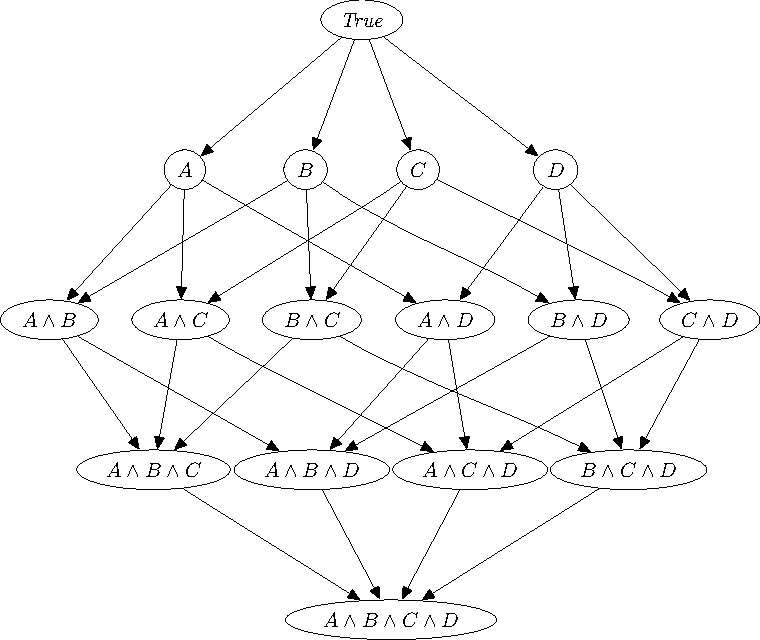
\includegraphics[width=8cm]{gfx/example_conjunctive_hypothesis_space}
\caption[An example of a conjunctive hypothesis space.]{An example of
  a conjunctive hypothesis space of four logical variables, $A$, $B$,
  $C$, and $D$.  All possible conjunctive hypotheses represented as
  nodes in a lattice with general-to-specific orderings represented by
  edges.}
\label{figure:example_conjunctive_hypothesis_space}
\end{figure}

\section{Concept Version Spaces}

Given a general-to-specific ordering of the entire hypothesis space,
Mitchell describes an efficient representation of all hypotheses that
match a given set of input examples, which he calls a \emph{version
  space}.  The implementation uses this very efficient version space
representation to keep track of all hypotheses in the conjunctive
hypothesis space that are consistent with factual knowledge.

%{\mbox{\autoref{figure:example_conjunctive_version_space}}} shows an
%example of a hypothesis version space.
%\begin{figure}
%\center
%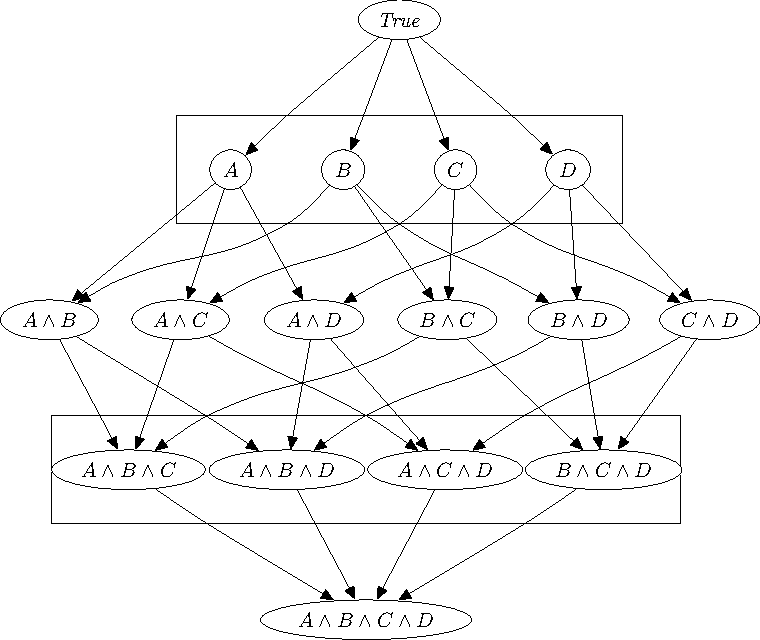
\includegraphics[width=8cm]{gfx/example_conjunctive_version_space}
%\caption[An example of a conjunctive hypothesis version space.]{An
%  example of a conjunctive hypothesis version space.}
%\label{figure:example_conjunctive_hypothesis_space}
%\end{figure}

%\begin{equation}
%{n\choose k} = \frac{n!}{k!(n-k)!}
%\end{equation}

\section{Hypothesizing Transframes from Preconditions}

In the model, planning is based on predicting the hypothetical effects
of resource actions.  In order to predict counterfactual
simultaneities, which can fill future slots of counterfactual
transitions, each historical resource activation transframe is
considered as input to a hypothesis version space concept learning
algorithm.

Equations\ \ref{equation:define_resource_precondition_symbols}
through\ \ref{equation:define_resource_transframe_remove_symbols}
define the precondition symbols, $a^*_E$, that can be used to
hypothetically predict the add and remove transframe symbols,
$a^*_{D^+}$ and $a^*_{D^-}$, for the general execution of the action
resource, $a^*$.
\begin{align}
\label{equation:define_resource_precondition_symbols}
  a^*_X &= \bigcup_{\epsilon \in a^*.\text{\tt{activation}}} [\text{pre}^{+}(\epsilon) \cup \text{pre}^{-}(\epsilon)] \\
\label{equation:define_resource_transframe_add_symbols}
  a^*_{D^+} &= \bigcup_{\epsilon \in a^*.\text{\tt{activation}}} \Delta^{+}(\epsilon) \\
\label{equation:define_resource_transframe_remove_symbols}
  a^*_{D^-} &= \bigcup_{\epsilon \in a^*.\text{\tt{activation}}} \Delta^{-}(\epsilon)
\end{align}
Equations\ \ref{equation:define_resource_hypothesis_space_first}
through\ \ref{equation:define_resource_hypothesis_space_last} define
the set of hypothesis spaces, $a_{\mathcal{H}}^{n*}$, for each action
resource, $a^{n*}$.
\begin{align}
\label{equation:define_resource_hypothesis_space_first}
                             a^{n*} &\in A^{n*} \\
                 a_{\mathcal{H}}^{n*} &\equiv \text{\emph{Resource hypothesis spaces}} \\
\label{equation:define_resource_hypothesis_space_last}
a^{n*}.\text{\tt{hypothesis-space}} &= a_{\mathcal{H}}^{n*} \\
\end{align}
Equations\ \ref{equation:define_hypothesis_space_first}
through\ \ref{equation:define_hypothesis_space_last} define a
conjunctive hypothesis space, $a_H^{n*}$, for an action resource,
$a^{n*}$.
\begin{align}
\label{equation:define_hypothesis_space_first}
                           a_H^{n*} &\in a_{\mathcal{H}}^{n*} \\
           a_H^{n*}.\text{\tt{add}} &\subseteq a^*_{D^+} \\
        a_H^{n*}.\text{\tt{remove}} &\subseteq a^*_{D^-} \\
                        a_{H_G}^{n*} &\equiv \text{\emph{Hypothesis space general hypotheses}} \\
       a_H^{n*}.\text{\tt{general}} &= a_{H_G}^{n*} \\
                        a_{H_S}^{n*} &\equiv \text{\emph{Hypothesis space specific hypotheses}} \\
\label{equation:define_hypothesis_space_last}
      a_H^{n*}.\text{\tt{specific}} &= a_{H_S}^{n*}
\end{align}
{\mbox{\autoref{figure:example_hypothesis}}} shows an example of a
hypothesis space.
\begin{figure}
\center
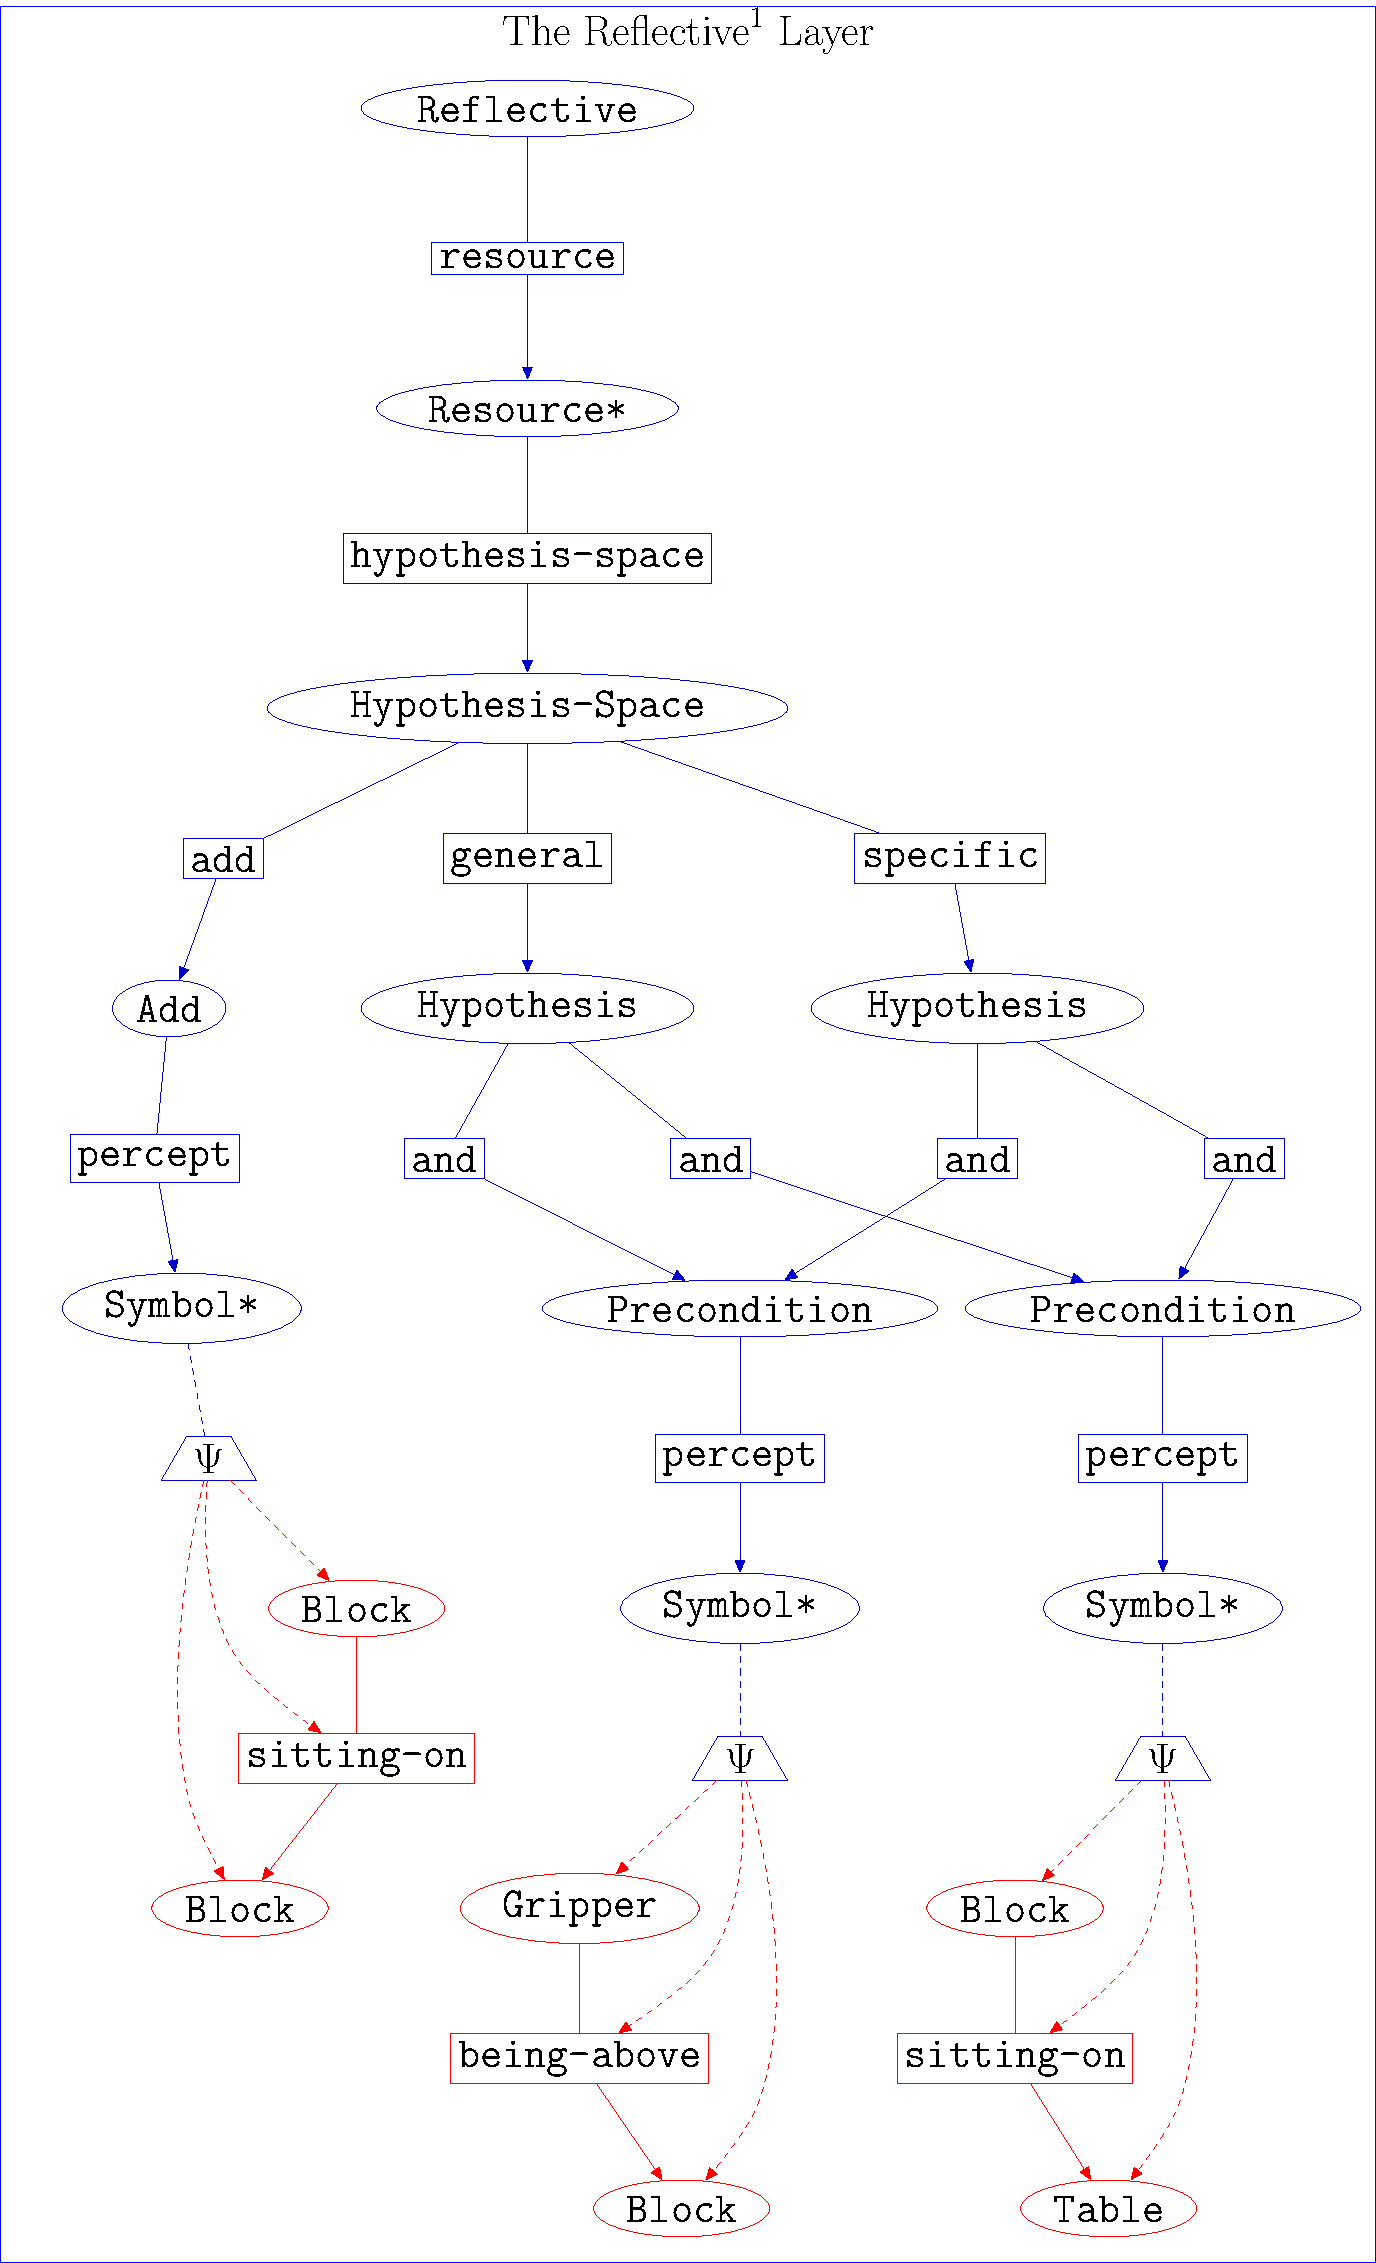
\includegraphics[width=12cm]{gfx/example_hypothesis}
\caption[An example of a resource activation hypothesis space.]{An
  example of a resource activation hypothesis space that can be used
  to predict the transframe addition of the percept of a block being
  on top of a block.}
\label{figure:example_hypothesis}
\end{figure}

\section{Decisions with Hypothesis Dependencies}

Hypothesis spaces are learned in order to predict counterfactual
transframes from factual preconditions and factual transframes.
However, when the time comes to make a prediction of a counterfactual
future, given factual preconditions, often the hypothesis spaces will
predict a number of potential outcomes with uncertainty.  This
uncertainty arises because, assuming that the choice of hypothesis
language allows for the expression of the correct hypothesis, not
enough factual examples have been seen in order to reduce the space to
this correct hypothesis.  Mitchell explains that if all of the current
possible hypotheses in the hypothesis space predict the same outcome,
this is guarenteed to be the correct outcome, again assuming that the
correct hypothesis is expressible in the hypothesis language.
However, often it is the case that the hypotheses make different
predictions.  If hypotheses are assumed to be equally likely, then
they can be counted and a probabilistic ratio can be computed.  I do
not make the assumption of equal likelihood of hypotheses, but some
assumption must be made in order for a decision to be made as to the
counterfactual outcome.

The important point is that when a decision is made, counterfactual
knowledge is created that depends on a specific subset of the
hypotheses in the hypothesis space remaining true.  In the
implementation, callbacks on the hypothesis-version-space learning
algorithm are used to propogate the removal of a hypothesis to the
counterfactual knowledge during learning and refining the hypothesis
space due to new factual knowledge.  This is only part of the response
to what will be later discussed as a type of \emph{expectation
  failure}, which creates a memory of the factual plan failure event
in addition to the refinement of the hypothesis space.

\section{Counterfactual Transframes}

When a counterfactual transframe is decidedly created based on
specific subsets of hypotheses in different hypothesis spaces, these
are kept track of as \emph{hypothesis dependencies} for each
counterfactual transframe.  Further, counterfactual transframes depend
on the future activation of a given set of resources.  These
\emph{activation dependencies} are also part of a counterfactual
transframe.
{\mbox{\autoref{figure:example_counterfactual_transframe}}} shows an
example of a counterfactual transframe with a hypothesis dependency as
well as an activation dependency.
\begin{figure}
\center
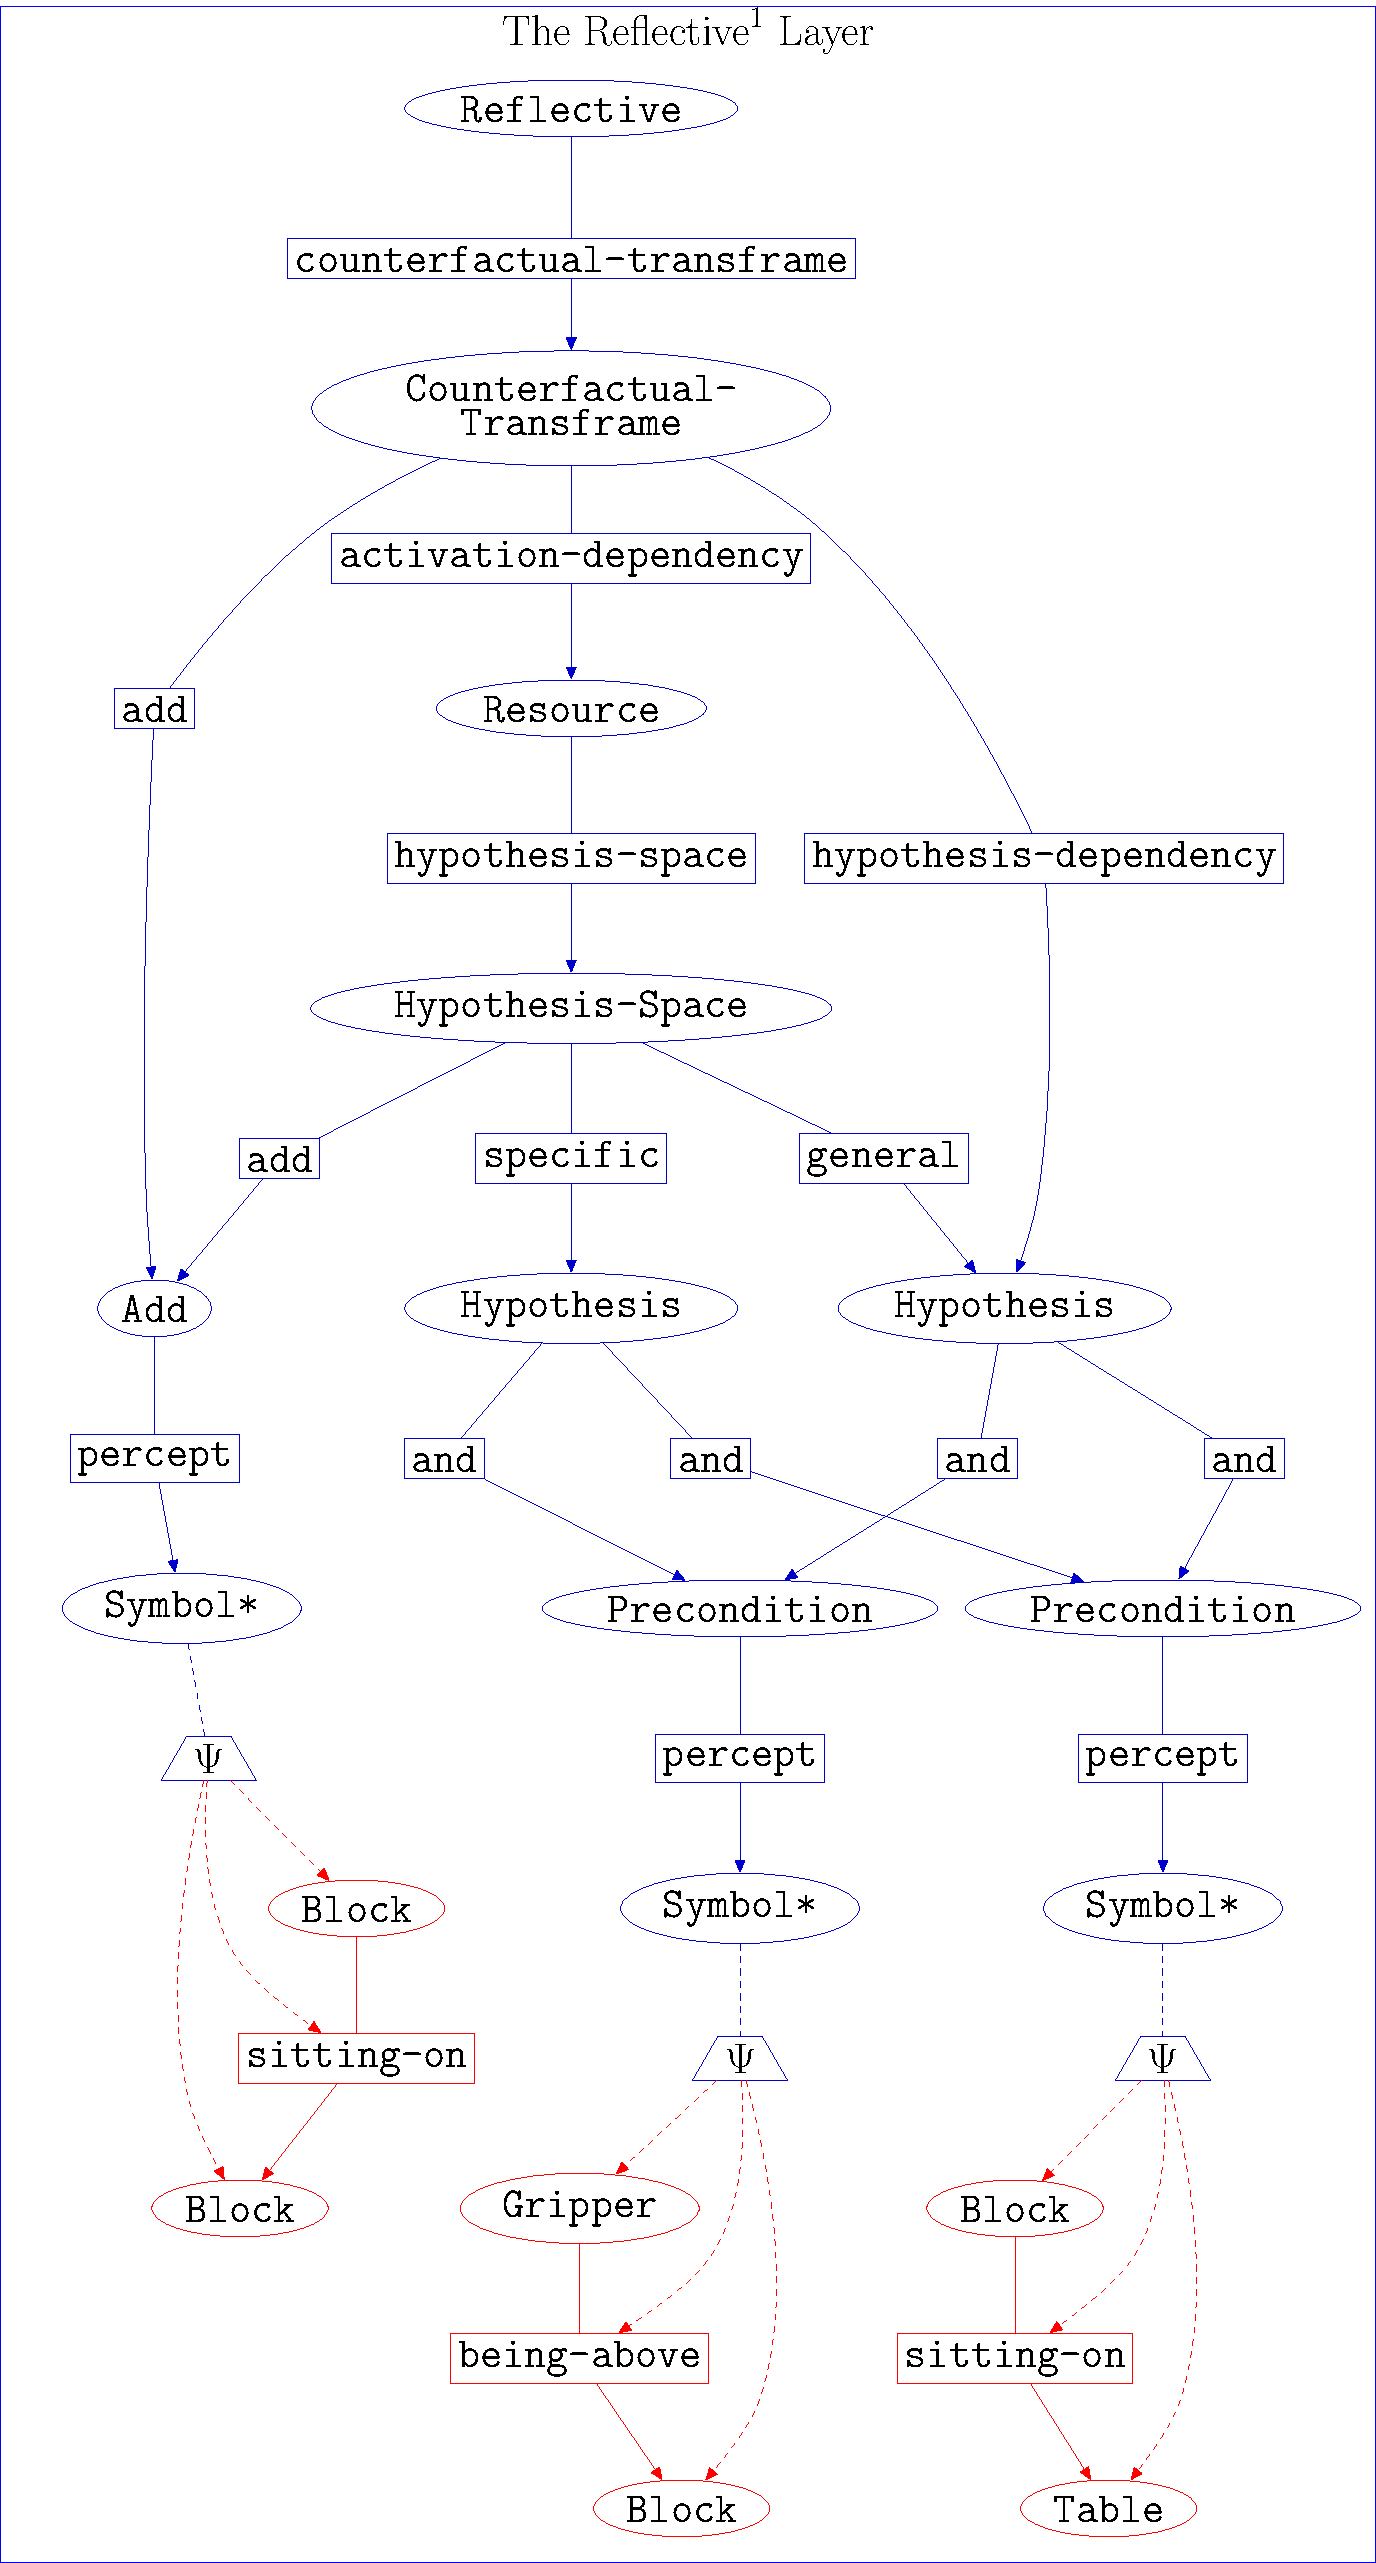
\includegraphics[width=12cm]{gfx/example_counterfactual_transframe}
\caption[An example of a counterfactual transframe.]{An example of a
  counterfactual transframe with a hypothesis dependency as well as an
  activation dependency.}
\label{figure:example_counterfactual_transframe}
\end{figure}

